% !TEX root = ../thesis.tex

%%%%%%%%%%%%%%%%%%%%%%%%%%%%%%%%%%%%%%%%%%%%%%%%%%%%%%%%%%%%%%%%%%%%%%%%%%%%%%%
% Chapter: Example Application
%%%%%%%%%%%%%%%%%%%%%%%%%%%%%%%%%%%%%%%%%%%%%%%%%%%%%%%%%%%%%%%%%%%%%%%%%%%%%%%
\chapter{Example Application: State Machine Monitoring}\label{Example Application}
In order to show how our managed data implementation works in practice, and in particular in terms aspect refactoring, we present a showcase in this Chapter.
The showcase consists of a very simple state machine application, which is inspired by Martin Fowler \ac{dsl}s book \cite{fowler2010domain}.
The same example is also presented in Enso papers as a showcase for its Object Grammar capabilities \cite{storm2012object}.

Consider the requirements of the state machine are the following: 
\begin{itemize}
	\item A state \texttt{Machine} consists of a number of named \texttt{State} declarations.

	\item Each \texttt{State} contains \texttt{Transitions} to other states, which are identified by a \texttt{name}, when a certain event happens.

	\item A \texttt{Transition} is identified by a certain \texttt{event}.
\end{itemize}

For simplicity, this example will be a very basic \textit{door state machine}, which includes three states \textbf{Open}, \textbf{Close} and \textbf{Locked} accompanied by their transitions: \textbf{open\_door}, \textbf{close\_door}, \textbf{lock\_door} and \textbf{unlock\_door} respectively.
Figure \ref{fig:State_machine} illustrates the door state machine.

\begin{figure}[H]
	\centering
  	\fbox{\includegraphics[width=.50\textwidth]{figures/State_machine.png}}
  	\caption{Basic door state machine}
  	\label{fig:State_machine}
\end{figure}

In order to implement the above we first need to define the models, next interpret the definition given a list of event and finally add any additional functionality (\textit{concern}) needed, for instance monitor the state of the door.

%%%%%%%%%%%%%%%%%%%%%%%%%%%%%%%%%%%%%%%%%%%%%%%%%%%%%%%%%%%%%%%%%%%%%%%%%%%%%%%
\section{Schemas definition}
First, we need to define all the models of the state machine program. 
The object diagram is illustrated in Figure \ref{fig:State_machine_object}.

\begin{figure}[H]
	\centering
  	\fbox{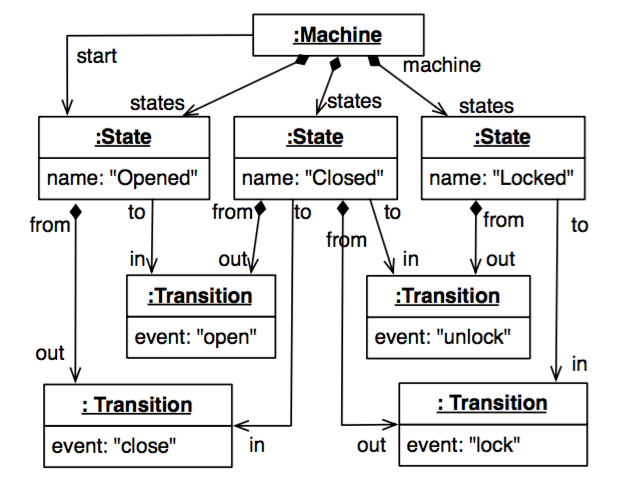
\includegraphics[width=.50\textwidth]{figures/State_machine_object_diagram.png}}
  	\caption{Basic door state machine object diagram}
  	\label{fig:State_machine_object}
\end{figure}

In our implementation we can define schemas using Java interfaces with a set of meta-data described with Java annotation.
Thus, as extracted from the requirements, we need \texttt{Machine} \ref{lst:Machine_Schema}, \texttt{State} \ref{lst:State_Schema}, and \texttt{Transition} \ref{lst:Transition_Schema} models (schemas).

%%%%%%%%%%%%%%%%%%%%%%%%%%%%%%%%%%%%%%%%%%%%%%%%%%%%%%%%%%%%%%%%%%%%%%%%%%%%%%%
\begin{sourcecode}[H]
	\begin{lstlisting}[language=Java,escapechar=|]
public interface Machine extends M {
	State start(State... startingState);

	State current(State... currentState);

	@Contain
	Set<State> states(State... states);
}
	\end{lstlisting}
	\caption{The Machine Schema}
	\label{lst:Machine_Schema}
\end{sourcecode}

As it can be seen in Listing \ref{lst:Machine_Schema}, for the \texttt{Machine} schema definition we need a \texttt{start}ing state, the \texttt{current} state of the machine and a set of \texttt{states} that the machine can be into at each time.
Note that, the \texttt{@Contain} annotation defines that the \texttt{states} field of this schema is part of the spine tree and it is not a cross-reference, but more about it in the implementation Chapter \ref{Schema Definition}.

%%%%%%%%%%%%%%%%%%%%%%%%%%%%%%%%%%%%%%%%%%%%%%%%%%%%%%%%%%%%%%%%%%%%%%%%%%%%%%%
\begin{sourcecode}[H]
	\begin{lstlisting}[language=Java,escapechar=|]
public interface State extends M {
	@Key
	String name(String... name);

	@Inverse(other = Machine.class, field = "states")
	Machine machine(Machine... machine);

	@Contain
	Set<Transition> out(Transition... transition);

	@Contain
	Set<Transition> in(Transition... transition);
}
	\end{lstlisting}
	\caption{The State Schema}
	\label{lst:State_Schema}
\end{sourcecode}

For the \texttt{State} definition, Listing \ref{lst:State_Schema}, we need a \texttt{name} field, which is representing name of the state. 
The \texttt{name} field has been annotated with the \texttt{@Key} annotation, which indicates that state names must be unique and the states field of Machine can be indexed by name.
Moreover, the schema includes a set of \texttt{in} and \texttt{out} \texttt{Transition}s.
Since those two fields are of type \texttt{Set}, that means that a field of the \texttt{Transition} schema has to be marked as key.
In this case is the name (line \ref{line:transition_key} Listing \ref{lst:Transition_Schema}).
Finally, the field \texttt{machine} represents which is the state machine that the current state part of. 
As it can be seen in the schema definition, listing \ref{lst:State_Schema}, the \texttt{machine} field has been annotated with \texttt{@Inverse}, which indicates that this field is a \textit{reference} to a field of an other schema, in this case this schema is the \texttt{Machine} schema and the field is the \texttt{states} field.
Thus, the \texttt{machine} field of \texttt{State} schema is a reference to \texttt{states} field of \texttt{Machine} schema.

%%%%%%%%%%%%%%%%%%%%%%%%%%%%%%%%%%%%%%%%%%%%%%%%%%%%%%%%%%%%%%%%%%%%%%%%%%%%%%%
\begin{sourcecode}[H]
	\begin{lstlisting}[language=Java,escapechar=|]
public interface Transition extends M {
	@Key 					|\label{line:transition_key}| 
	String event(String... event);

	@Inverse(other = State.class, field = "out")
	State from(State... from);

	@Inverse(other = State.class, field = "in")
	State to(State... to);
}
	\end{lstlisting}
	\caption{The Transition Schema}
	\label{lst:Transition_Schema}
\end{sourcecode}

Finally, for the \texttt{Transition} schema definition, Listing \ref{lst:Transition_Schema}, all we need is an \texttt{event} which represents the event of the transition and it is also the \textbf{key}.
Additionally, the \texttt{from} and \texttt{to} states represent the state that the machine changes from and to respectively.
However, those are just reference to the \texttt{State} schema, Listing \ref{lst:State_Schema}, to the \texttt{in} and \texttt{out} fields respectively, since they are defined with the \texttt{@Inverse} annotation.

%%%%%%%%%%%%%%%%%%%%%%%%%%%%%%%%%%%%%%%%%%%%%%%%%%%%%%%%%%%%%%%%%%%%%%%%%%%%%%%
\section{Factory definition}
Since we have our schemas now we need a way to build instances of managed objects of those schemas. 
For Java to create the three schemas as managed data we need to define a factory, which will be the one that creates managed data instances (managed objsects) for each of these schemas \ref{lst:StateMachineFactory}.
Note that those definitions work as \texttt{Constructors} of managed objects.

\begin{sourcecode}[H]
	\begin{lstlisting}[language=Java,escapechar=|]
public interface StateMachineFactory {
	Machine Machine();  // builds a Machine managed object
	State State(); 			// builds a State managed object
	Transition Transition(); // builds a Transition managed object
}
	\end{lstlisting}
	\caption{The StateMachine Factory}
	\label{lst:StateMachineFactory}
\end{sourcecode}

%%%%%%%%%%%%%%%%%%%%%%%%%%%%%%%%%%%%%%%%%%%%%%%%%%%%%%%%%%%%%%%%%%%%%%%%%%%%%%%
\section{Basic Data Manager}
As it is mentioned, in order to interpret and manage the defined data we need data managers. 
Our implementation includes the definition of a \texttt{Basic data manager} that is responsible of making a schema definition to an instance of \textit{managed object}.
However, in order to make the \textit{managed object} it needs its schema definition (the interfaces that define the schemas) and the schema factory (the interface that defines the constructors of the schemas).

%%%%%%%%%%%%%%%%%%%%%%%%%%%%%%%%%%%%%%%%%%%%%%%%%%%%%%%%%%%%%%%%%%%%%%%%%%%%%%%
\subsection{A simple without concerns program}
In the case of a simple program without any concerns, we have to use our managed data to define the state machine and then interpret it.
The definition of the door state machine is given in Listing \ref{lst:Door_state_machine} in Java.

In practice, we need the basic data manager to have a mechanisms that interprets the managed object that comply the \texttt{stateMachineSchema}, shown in Line \ref{line:state_meaning_full_code}.
A a simple interpreter for the state machine is shown in Line \ref{line:state_machine_interpreter}.
As it can be seen, the schemas factory is used to create managed objects and the \textit{wiring} of the fields is done automatically by the data manager who is responsible for the managed object interpretation.

\begin{sourcecode}
	\begin{lstlisting}[language=Java, escapechar=|]
public class StateMachineExample {
	public static void main(String[] args) {
		final Schema schemaSchema = ...; |\label{line:state_schemaSchema}|
		final Schema stateMachineSchema = ....; |\label{line:state_schemaMachineSchema}|

		final BasicDataManager basicDataManagerForStateMachines = 
				new BasicDataManager(StateMachineFactory.class, stateMachineSchema);  |\label{line:state_meaning_full_code}|
		final StateMachineFactory stateMachineFactory = basicDataManagerForStateMachines.make();

		final Machine doorStateMachine = stateMachineFactory.Machine(); |\label{line:state_machine_creation_basic}|

		final State openState = stateMachineFactory.State(OPEN_STATE);
		openState.machine(doorStateMachine);

		final State closedState = stateMachineFactory.State(CLOSED_STATE);
		closedState.machine(doorStateMachine);

		final State lockedState = stateMachineFactory.State(LOCKED_STATE);
		lockedState.machine(doorStateMachine);

		final Transition closeTransition = stateMachineFactory.Transition(CLOSE_TRANSITION);
		closeTransition.from(openState);
		closeTransition.to(closedState);

		final Transition openTransition = stateMachineFactory.Transition(OPEN_TRANSITION);
		openTransition.from(closedState);
		openTransition.to(openState);

		final Transition lockTransition = stateMachineFactory.Transition(LOCK_TRANSITION);
		lockTransition.from(closedState);
		lockTransition.to(lockedState);

		final Transition unlockTransition = stateMachineFactory.Transition(UNLOCK_TRANSITION);
		unlockTransition.from(lockedState);
		unlockTransition.to(closedState);

		doorStateMachine.start(closedState);

		interpretStateMachine(doorStateMachine, new LinkedList<>(Arrays.asList(
		        LOCK_TRANSITION,
		        UNLOCK_TRANSITION,
		        OPEN_TRANSITION)));
	}
}

private static void interpretStateMachine(Machine stateMachine, List<String> commands) { |\label{line:state_machine_interpreter}|
    stateMachine.current(stateMachine.start());
    for (String event : commands) {
        for (Transition trans : stateMachine.current().out()) {
            if (trans.event().equals(event)) {
                stateMachine.current(trans.to());
                break;
            }
        }
    }
}   
	\end{lstlisting}
	\caption{Door state machine}
	\label{lst:Door_state_machine}
\end{sourcecode}

%%%%%%%%%%%%%%%%%%%%%%%%%%%%%%%%%%%%%%%%%%%%%%%%%%%%%%%%%%%%%%%%%%%%%%%%%%%%%%%
\section{Monitoring and notification concerns}
Consider now the case which we want to add some concerns at the previous door state machine implementation.
A simple concern would be a \textit{monitoring} concern, which will log every change in the current state of the state machine.
Another concern would be a \textit{notification} which would be enabled when a specific state is set to the machine.

Suppose, for this example, the system has to notify someone in case the door is opened.
In the case that the door opens, the \textbf{Open} state has set to the current state to the machine, then we want to notify someone by e-mail.
That looks similar to the \textit{monitoring} concern yet, in this case the notification is a specific action; send an e-mail in case the door is open.

\begin{figure}[H]
	\centering
  	\fbox{\includegraphics[width=.50\textwidth]{figures/State_machine_danger.png}}
  	\caption{Simple door state machine: notify closed door}
  	\label{fig:State_machine_danger}
\end{figure}

In order to implement those concerns we need a mechanism that continuously monitors the changes (transitions) of the machine's \texttt{current} state and react accordingly.
In a traditional way this would lead to scattered \textit{monitoring} and \textit{notification} code inside the interpretation method or the models themselves (the machine model).
However, in managed data there are data managers for that purpose.
A data manager can implement concerns as modular aspects without crosscut code to the components.
Therefore, by implementing our concerns with data managers we can keep the interpretation and model definition code, shown in Listing \ref{lst:Door_state_machine}, modular.

%%%%%%%%%%%%%%%%%%%%%%%%%%%%%%%%%%%%%%%%%%%%%%%%%%%%%%%%%%%%%%%%%%%%%%%%%%%%%%%
\subsection{Observable Data Manager}
In order to \textit{observe} for changes in the current state of our door state machine we need a data manager that observes changes in the managed object.
In particular, the \texttt{Machine}'s current \texttt{State}.
This data manager creates concrete managed objects, namely \textit{observable managed object} with which one attach observers that will be notified in case of changes.

%%%%%%%%%%%%%%%%%%%%%%%%%%%%%%%%%%%%%%%%%%%%%%%%%%%%%%%%%%%%%%%%%%%%%%%%%%%%%%%
\subsection{Monitor and notify concerns}
In the example, the observers are the concerns, which are \textit{monitoring} and \textit{notification} by e-mail in case of opened door. 
The definition of those concerns is given in Listing \ref{lst:StateMachineMonitoring}.

\begin{sourcecode} [H]
	\begin{lstlisting}[language=Java, escapechar=|]
public class StateMachineMonitoring {
    public static void monitor(Object obj, String field, Object value) {
        if (field.equals("current")) {
            logger.log(" > Current state changed to " + ((State) value).name());
        }
    }

    public static void notify(Object obj, String field, Object value) {
        if (field.equals("current") && ((State) value).name().equals(OPEN_STATE)) {
            if (EmailSender.send("Danger!", "Someone just opened the door!")) {
            	logger.notify(" > Danger e-mail sent!.");
            }
        }
    }
}
	\end{lstlisting}
	\caption{Door state machine concerns definition}
	\label{lst:StateMachineMonitoring}
\end{sourcecode}

Since there is an observable data manager and the concerns implemented in a separate and reusable module, completely unrelated to our logic code, it is still needed to be integrate them in the door state machine original code.
The integration code is presented in Listing \ref{lst:StateMachineMonitoringConcerns}.
The only part that it changes is the line \ref{line:state_machine_creation_basic} of the original code, in which the data manager of the \texttt{Machine} managed object has changed to the new observable data manager.
Additionally, the concerns are attached to the machine object very easily, as can be seen in lines \ref{line:state_machine_monitor} and \ref{line:state_machine_notify} of Listing \ref{lst:StateMachineMonitoringConcerns}.


\begin{sourcecode} [H]
	\begin{lstlisting}[language=Java, escapechar=|]
...
// State Machine monitoring
final ObservableDataManager observableDataManager = 
			new ObservableDataManager(StateMachineFactory.class, stateMachineSchema);

final StateMachineFactory observableStateMachineFactory = observableDataManager.make();

// Door State Machine definition, with observable data manager
final Machine doorStateMachine = observableStateMachineFactory.Machine();

// Add monitoring and notification concerns
((Observable) doorStateMachine).observe(StateMachineMonitoring::monitor); |\label{line:state_machine_monitor}|
((Observable) doorStateMachine).observe(StateMachineMonitoring::notify);  |\label{line:state_machine_notify}|
...
	\end{lstlisting}
	\caption{Door state machine with concerns}
	\label{lst:StateMachineMonitoringConcerns}
\end{sourcecode}

By running the program with the three commands \texttt{LOCK\_TRANSITION}, \texttt{UNLOCK\_TRANSITION} and \texttt{OPEN\_TRANSITION}, the output is presented in Listing \ref{lst:StateMachineMonitoringConcernsOutput} along with an e-mail sent.
\lstdefinestyle{Bash} {
    backgroundcolor=\color{white},
    basicstyle=\scriptsize\color{black}\ttfamily
}

\begin{sourcecode} [H]
	\lstset{numbers=none}
	\begin{lstlisting}[style=Bash]
> Current state changed to Closed
> Current state changed to Locked
> Current state changed to Open
> Danger e-mail sent!
	\end{lstlisting}
	\caption{Door state machine with concerns: output}
	\label{lst:StateMachineMonitoringConcernsOutput}
\end{sourcecode}

The basic data manager allows to just build managed object, but the observable data manager provided with the functionality of attaching concerns in the managed objects after an specified observed event.
Concluding, that example just presented a modular solution of \ac{ccc} without scattering and tangling code in the components.
